\section*{Dati e risultati}

\subsection*{Rilevatore di picchi}

In questa sezione ci occuperemo di verificare il corretto funzionamento di un circuito rilevatore di picchi costruito con un diodo 1N4007.
Il circuito che abbiamo utilizzato è schematizzato in Figura \ref{fig:circuito_peak}.
In questa configurazione abbiamo impostato che il valore di capacità ($C$) fosse di $1\,\si{\micro\farad}$, mentre il valore della resistenza $R_2$ fosse di $1\,\si{\kilo\ohm}$. Ricordiamo che sul valore della capacità abbiamo un incertezza nominale dell'$1\,\%$, mentre sulla resistenza vi è un errore nominale del $5\,\%$.
Il circuito è stato alimentato con una differenza di potenziale picco-picco in entrata di $10\,\si{\volt}$ ad una frequenza di $100\,\si{\hertz}$.

Quindi per verificare il corretto funzionamento del nostro rilevatore di picchi visualizziamo la tensione in uscita ($V\ped{out}$) e ne studiamo l'andamento al variare di $C$ e della resistenza $R_1$.
Aggiungiamo che per semplificare le operazioni abbiamo deciso di variare la resistenza $R_1$ mantenendo costante la capacità, e di seguito variare $C$ mantenendo costante $R_1$.
Riportiamo in Figura \ref{fig:capacita} e \ref{fig:resistenza} gli andamenti della
tensione in uscita ($V\ped{out}$) al variare di $C$ e di $R_1$.

Infine vogliamo evidenziare che nel caso in cui si invertisse la polarità del diodo si noterebbe che il segno dei
picchi in output si inverte, come abbiamo testato durante l'esperienza.

\begin{SCfigure}[0.5][t]
    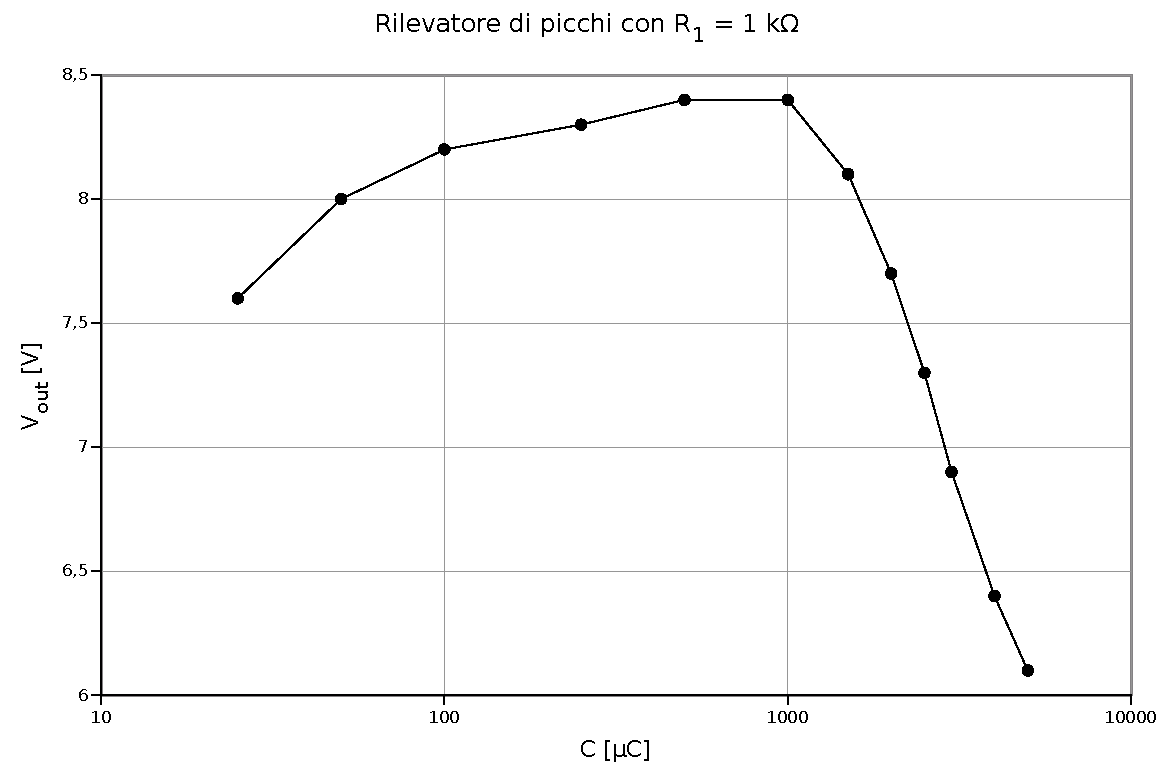
\includegraphics[scale=0.68]{capacita.pdf}
    \caption{Questo grafico illustra il valore di tensione in uscita del circuito illustrato in Figura \ref{fig:circuito_peak} in funzione della resistenza $R_1$ applicata, mantenendo costante la capacità. Gli errori sulle misure non sono riportati in quanto sono troppo piccoli per essere visibili. Inoltre è possibile osservare che vi è un picco in corrispondenza del valore di resistenza $R_1$ di $1\,\si{\kilo\ohm}$, ovvero quando $R_1$ è uguale ad $R_2$. Infine evidenziamo che la retta delle ascisse è in scala logaritmica al fine di rendere più leggibile il grafico.}
    \label{fig:capacita}
\end{SCfigure}

\begin{SCfigure}[0.5][t!]
    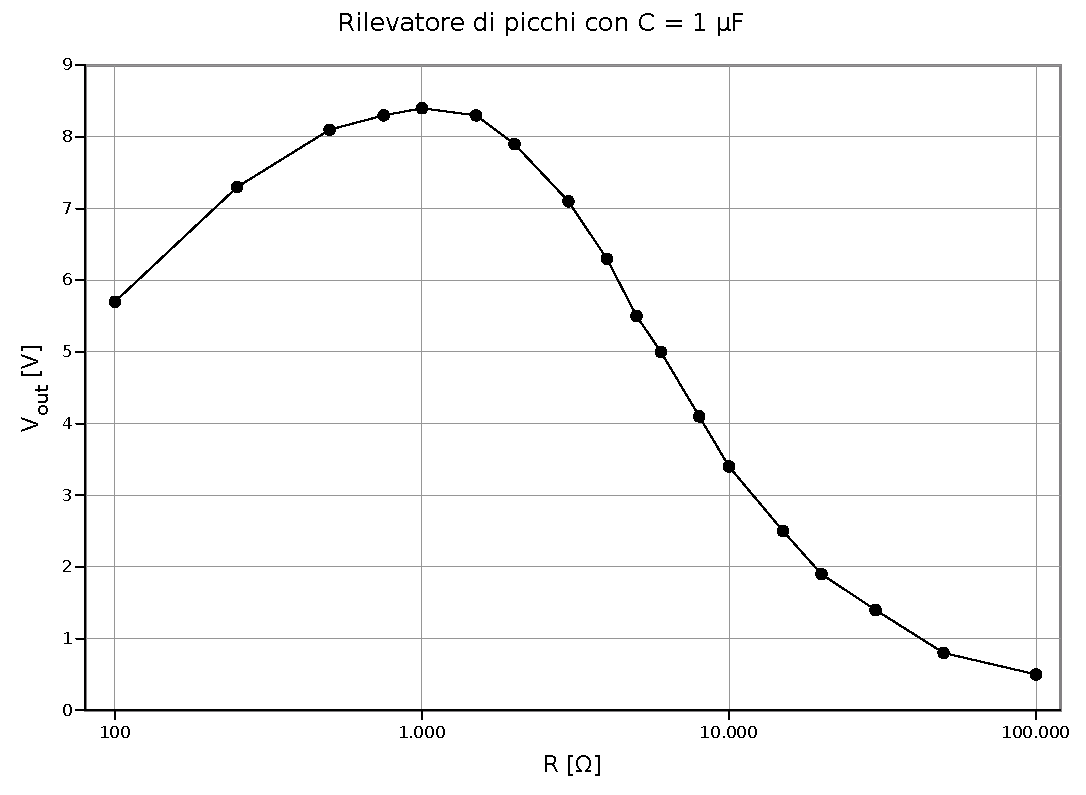
\includegraphics[scale=0.68]{resistenza.pdf}
    \caption{Questo grafico illustra il valore di tensione in uscita del circuito illustrato in Figura \ref{fig:circuito_peak} in funzione della capacità $C$ applicata, mantenendo costante la resistenza $R_1$. Gli errori sulle misure non sono visibili in quanto troppo piccoli per essere visualizzati. Infine possiamo notare la presenza di un picco in prossimità del valore di $C$ di $1\,\si{\milli\farad}$. Infine evidenziamo che la scala dell'asse delle ascisse è logaritmica.}
    \label{fig:resistenza}
\end{SCfigure}

\subsection*{Diodo Zener}

In questa seconda sezione vogliamo studiare la caratteristica $I-V$ in polarizzazione inversa del diodo Zener, modello XZY85C10 ed il suo uso come stabilizzatore di tensione.
Per studiarne la caratteristica $I-V$ abbiamo applicato ai capi del diodo Zener una tensione DC variabile. 
Durante lo studio della caratteristca $I-V$ del diodo abbiamo tenuto conto della potenza massima dissipabile dal diodo. Infatti abbiamo fatto attenzione che il prodotto tensione-corrente non superasse mai la potenza ($W$) di $1\,\si{\watt}$, che è il valore massimo sopportabile dal nostro diodo.
I valori ottenuti sono riportati nel grafico in Figura \ref{fig:caratteristica_I-V}.

Inoltre abbiamo calcolato la resistenza dinamica ($R_d$) del diodo sfruttando la seguente relazione:

\begin{equation}
	R_d \,=\, \frac{\Delta V}{\Delta I} \,=\, 14.2\,\pm\,0.1 \,\,\si{\ohm}
\end{equation}

%14.209713510314533
%0.106189350778691

dove $\Delta V$ indica una differenza di potenziale e $\Delta I$ indica la differenza di intensità di corrente corrispondente.
Per calcolare questo valore, abbiamo esegiuto la regressione lineare sui punti del grafico (Figura \ref{fig:caratteristica_I-V})
oltre la tensione di breakdown del diodo, essendo l'andamento una retta quasi perfetta. Possiamo notare che la resistenza dinamica $R_d$ non è altro che l'inverso del coefficiente angolare della retta plottata. \\

\begin{SCfigure}[0.5][t]
   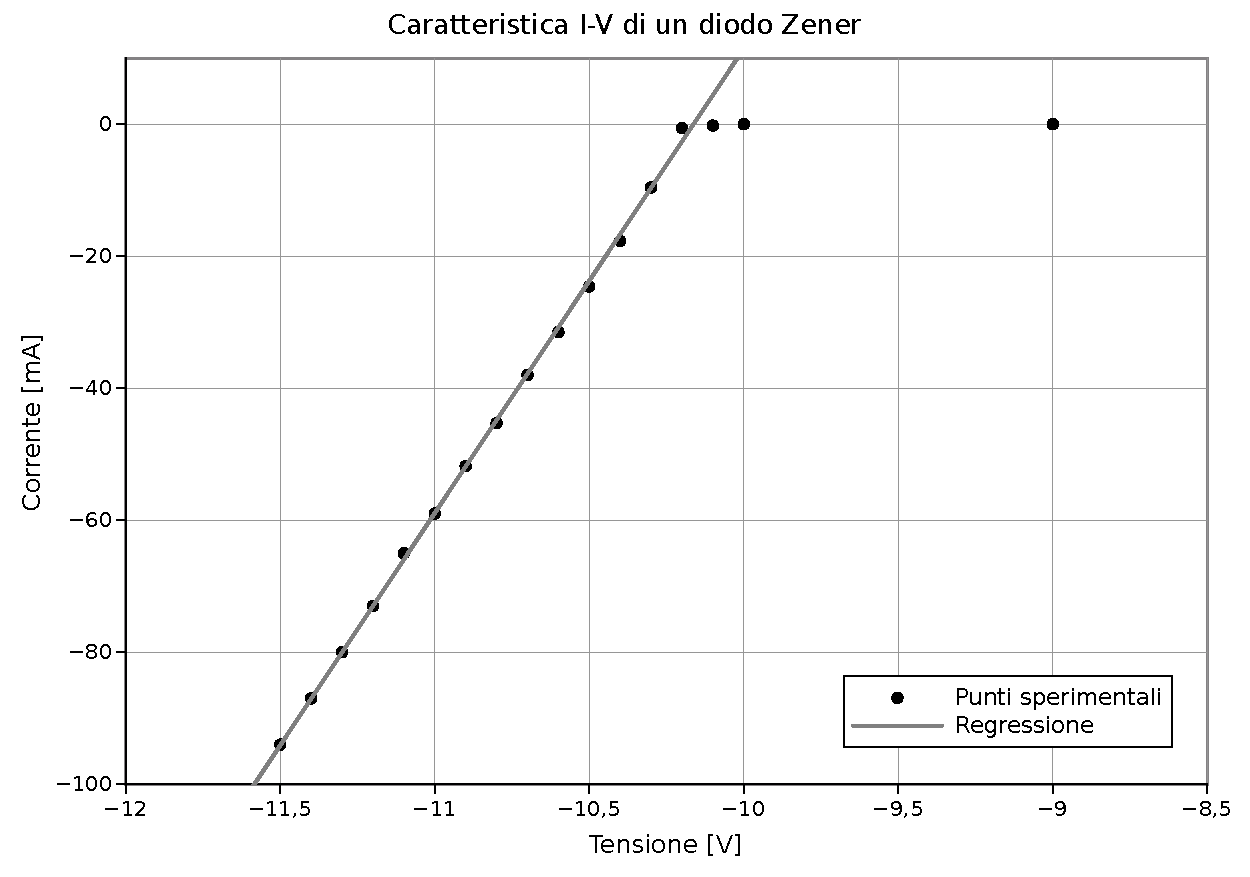
\includegraphics[scale=0.68]{cara_zener.pdf}
    \caption{Questo grafico mostra la caratteristica $I-V$ del diodo Zener, modello modello XZY85C10. In queso caso le incertezze sui dai sono troppo piccole per essere visualizzate. Possiamo osservare che la tensione di breakdown è di circa $-10.2\,\si{\volt}$. Infine la retta di fit per i dati oltre la tensione di breakdown è una retta quasi perfetta.}
    \label{fig:caratteristica_I-V}
\end{SCfigure}

Ottenute queste informazioni su questo modello di diodo Zener ci siamo proposti di determinare sperimentalmente, studiandone la caratteristica $I-V$, il range di funzionamento di tale componente elettronico se usato come stabilizzatore di tensione.
A tal fine abbiamo sfruttato il circuito illustrato in Figura \ref{fig:circuito_zener} che è stato alimentato con il generatore di tensione DC e la resistenza ($R$) applicatavi è di $1\,\si{\kilo\ohm}$.
I risultati da noi ottenuti sono riportati nel grafico in Figura \ref{fig:stab_tensione}.

\begin{SCfigure}[0.5][b!]
    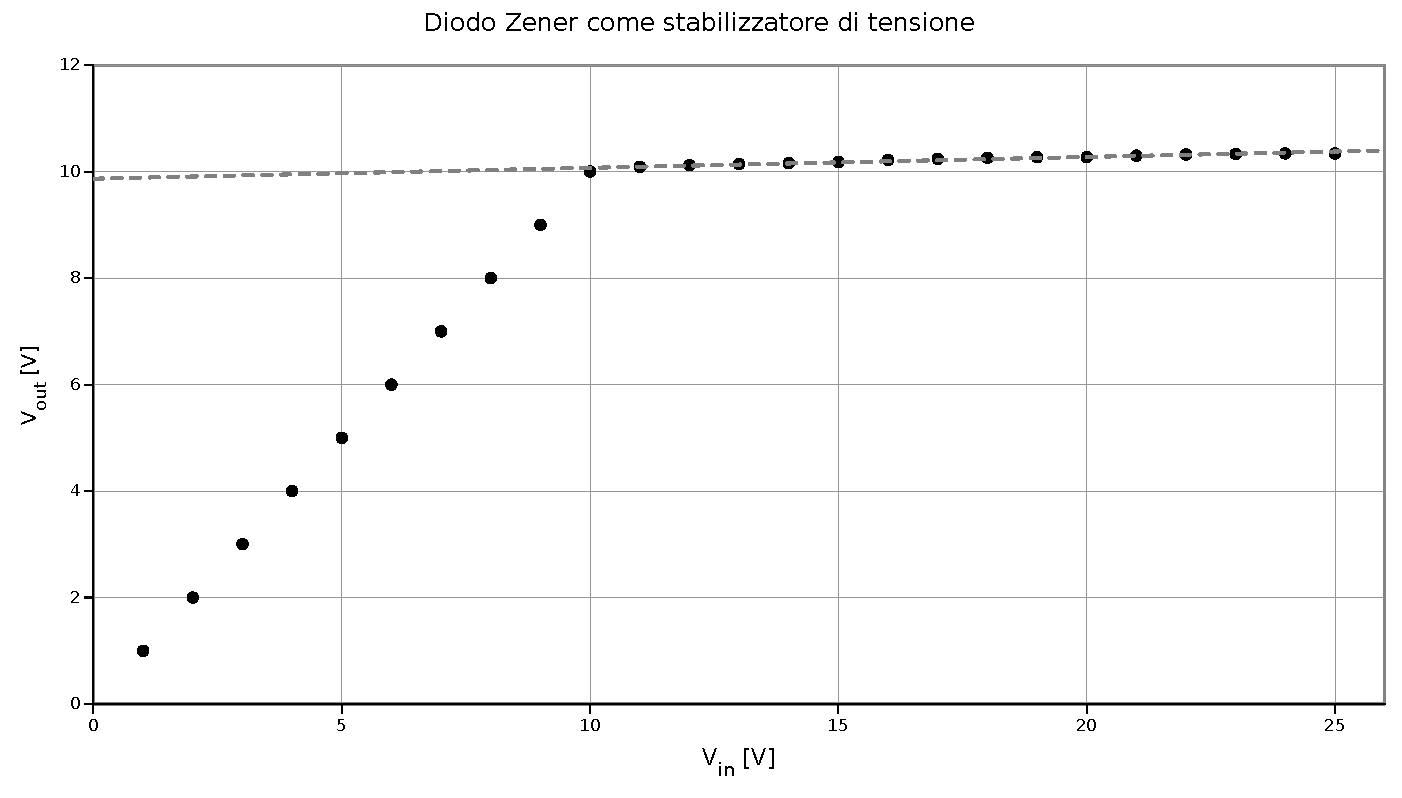
\includegraphics[scale=0.68]{stab.pdf}
    \caption{Questo grafico mostra la caratteristica $I-V$ del nostro stabilizzatore di tensione. Le incertezze sulle misure non sono visibili in quanto troppo piccole pere essere plottate. Come si può osservare il diodo Zener stabilizza la tensione in ingresso per valori di differenza di potenziale uguali o superiori a $10\,\si{\volt}$. Al di sotto della tensione di $10\,\si{\volt}$ il diodo si comporta come un circuito aperto.}
    \label{fig:stab_tensione}
\end{SCfigure}

Infine vogliamo calcolare il rapporto di stabilizzazione ($\chi$) sia teorico che sperimentale e verificarne la compatibilità.
Il rapporto di stabilizzazione teorico è stato ricavato dal fit sui dati mostrato in Figura \ref{fig:stab_tensione}.

\begin{equation}
	\chi\ped{exp} \,=\, \frac{\Delta V\ped{out}}{\Delta V\ped{in}} \,=\, 0.020\,\pm\,0.001
	\label{eq:c_exp}
\end{equation}

\begin{equation}
	\chi\ped{teo} \,=\, \frac{R_d}{R\,+\,R_d} \,=\, 0.0140\,\pm\,0.0006
	\label{eq:c_teo}
\end{equation}
